\chapter{Conception}

Le programme développé ici est supposé répondre à un besoin bien précis, c'est-à-dire l'accessibilité d'une ressource bien définie et son utilisation, que ce soit par un utilisateur humain ou par une intelligence artificielle développée spécifiquement pour le jeu souhaité. La première partie de ce projet a donc été dédiée à la conception de ce projet par les besoins d'un utilisateur quel qu'il soit.\\

\section{Diagrammes de séquence}

Ci-dessous sont détaillés les scénarios d'usage du logiciel, ainsi que leurs diagrammes de séquence associés. C'est l'ensemble de ces éléments qui nous a permis par la suite de cerner le cœur de ce qui est attendu à la fin de ce sujet.\\

Nous nommerons ici "entité" l'utilisateur: en effet, en plus d'un utilisateur humain, administrateur ou non, une intelligence artificielle devrait également être en mesure d'accéder à notre service afin d'instancier une partie ou rejoindre une partie existante, se confrontant alors à une autre intelligence artificielle ou à un joueur déjà présent en jeu.

\newpage
\subsection{Premier cas d'utilisation: créer une partie d'un jeu}	
	
	\begin{figure}[!ht]
		\center
		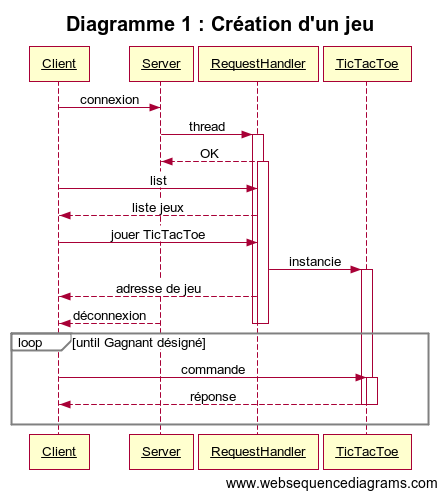
\includegraphics[scale=0.7]{images/sequence/diagramme_scenario1.png}
		\caption{Le premier cas d'utilisation, basique}
	\end{figure}
	
	\underline{Description}\\
	
	\textit{Une entité souhaite jouer à un jeu. Elle lance donc le client, qui lui permet de se connecter 
		au serveur. Elle entre la commande “list” qui lui permet de voir quels jeux sont disponibles. 
		Parmi eux, elle choisit le TicTacToe, qui est alors instancié du fait qu'aucune partie n'est active. Le serveur lui renvoie l'adresse de jeu, à laquelle l'entité se pourra se connecter que si suffisamment de joueurs souhaitent participer.}\\
	
	\vspace{3em}
	Ce cas d'utilisation pose les bases de l'utilisation de notre serveur: on l'utilise principalement pour jouer, et on attend que suffisamment de joueurs soient en attente pour ce jeu afin d'en instancier une.
	\newpage
	
	\subsection{Deuxième cas d'utilisation: rejoindre une partie existante}
	\begin{figure}[!ht]
		\center
		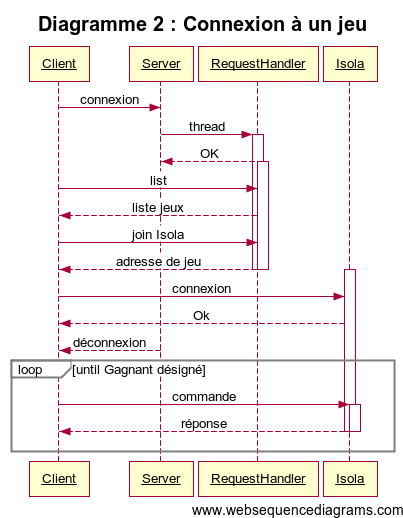
\includegraphics[scale=0.7]{images/sequence/diagramme_rejoindre.png}
		\caption{Rejoindre une partie}
	\end{figure}
	
	\underline{Description}\\
	
	\textit{Une entité souhaite jouer à un jeu. Elle lance donc le client, qui lui permet de se connecter 
		au serveur. Elle entre la commande “list” qui lui permet de voir quels jeux sont disponibles. 
		Parmi eux, elle choisit de jouer à l'Isola. Des parties étant déjà en cours, le serveur lui renvoie l'adresse d'une des parties, à laquelle l'entité se connecte pour ensuite jouer à l'Isola.}\\
	
	\vspace{3em}
	Ce cas d'utilisation introduit la notion non plus de création d'une instance de jeu, mais bien de connexion à une partie existante. Il faut donc définir des moyens de contrôler et de retenir les jeux étant actuellement instanciés pour pouvoir effectuer la connexion entre le client et le jeu en question.
	\newpage
	
	\subsection{Troisième cas d'utilisation: ajouter un jeu sur le serveur}
	\begin{figure}[!ht]
		\center
		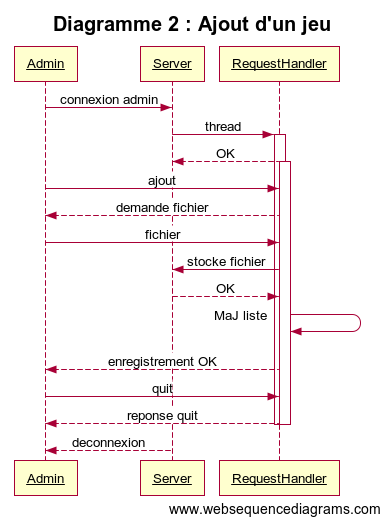
\includegraphics[scale=0.7]{images/sequence/diagramme_ajout.png}
		\caption{Ajout d'un jeu}
	\end{figure}
	
	\underline{Description}\\
	
	\textit{Un administrateur se connecte au service en ligne, via un pseudonyme et mot de passe associés. Il ajoute ensuite un jeu via la commande associée, et le fichier du jeu lui est demandé: il le choisir, et valide son choix. Il choisit un nom pour le jeu choisi, et le serveur stocke ledit fichier dans ses données, mettant  à jour la liste des jeux disponibles. Une fois l'enregistrement effectué, l'administrateur entre la commande 'quit' et se voit déconnecté du serveur.}\\
	
	\vspace{3em}
	
	Ce troisième cas d'utilisation introduit un autre acteur possible, soit l'administrateur. Entrent en compte des problèmes de sécurité liés au statut privilégié, l'enregistrement de fichiers et la saisie de celui-ci.
	\newpage
	
	\subsection{Quatrième cas d'utilisation: quitter une partie en cours}
	\begin{figure}[!ht]
		\center
		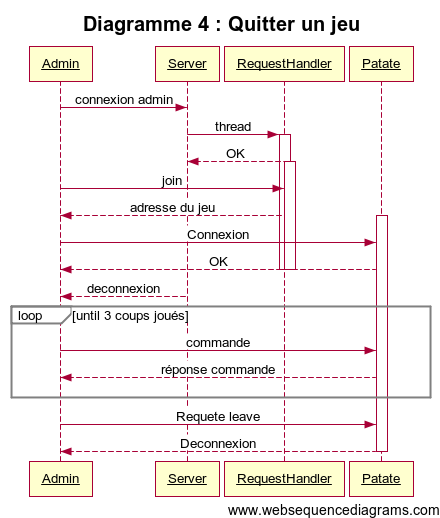
\includegraphics[scale=0.7]{images/sequence/diagramme_leave_cas1.png}
		\caption{Quitter une partie}
	\end{figure}
	
	\underline{Description}\\
	
	\textit{Une entité souhaite participer à une partie. Elle entre donc la commande 'join Patate', qui lui permettra de se connecter à une partie actuellement en cours de la Patate chaude. L'adresse du jeu lui est renvoyée et elle s'y connecte. Cependant, au bout de trois coups joués, elle se rend compte qu'elle ne souhaite pas continuer à jouer. Elle entre donc la commande 'leave', et se voit immédiatement déconnectée du jeu en cours.}\\
	
	\vspace{3em}
	
	Lorsque l'on joue à un jeu, il est aussi bénéfique de savoir comment le quitter, pour des raisons diverses. Cependant, ce cas d'utilisation ne concerne pas vraiment le serveur développé par nos soins: en effet, une fois connecté au jeu, l'interaction avec le \textit{software} devient nulle, et la commande permettant de quitter une partie devrait alors être partie intégrante du système de jeu.
	\newpage

